\documentclass{article}
\usepackage[english]{babel}
\usepackage[utf8]{inputenc}
\usepackage[T1]{fontenc}
\usepackage{graphicx}
\usepackage[colorinlistoftodos]{todonotes}
\usepackage[colorlinks=true, allcolors=tudelftblue]{hyperref} %sets hyperlink colour
\usepackage{caption}
\usepackage{subcaption}
\usepackage{xcolor}
\usepackage{roboto} % for Roboto Slab font
\usepackage{float}
\usepackage{titling} 
\usepackage{blindtext}\usepackage{titlesec}
\usepackage[square,sort,comma,numbers]{natbib}
\usepackage[colorinlistoftodos]{todonotes}
\usepackage{tikz}
\usepackage{geometry}
\usepackage{sectsty}
\usepackage{amsmath}
\usepackage{tikzpagenodes}
\usepackage{booktabs}
\usepackage{longtable}
\usepackage{titlesec}
\usepackage{listings}
\definecolor{tudelftdarkblue}{RGB}{0,0,0}
\definecolor{tudelftcyan}{RGB}{209,65,36}
\definecolor{tudelftblue}{RGB}{99, 102, 106}
\geometry{a4paper, margin=2cm}
\allsectionsfont{\color{black}} %sets colour for all headers
\usepackage{helvet}
\renewcommand{\familydefault}{\sfdefault}
\sectionfont{\fontfamily{RobotoSlab-TLF}\selectfont}
%%%%%%%%%%%%%%%%%%%%%%%%%%%%%%%%%%%%%%%%%%%%%%%%%%%%%%%%%
\begin{document}

\begin{titlepage}
    \fontfamily{RobotoSlab-TLF}\selectfont 

    \begin{center}
%%%%%%%%%%%%%%%%%%%%%%%%%%%%%%%%%%%%%%%%%%%%%%%%%%%%%%%%%%UNCOMMENT THE FOLLOWING FOR LESS "PLAIN" TITLE PAGE (SELECT WITH MOUSE AND PRESS CTRL AND /)

    % \begin{tikzpicture}[remember picture,overlay]
    %     % Set seed for random number generator
    %     \pgfmathsetseed{4}
    %     % Define the text area to avoid
    %     \path (current page text area.south west) rectangle (current page text area.north east);
    %     % Adding circles spread over the entire page
    %     \foreach \x in {1,...,1000}
    %         \draw[tudelftdarkblue] (current page.south west) ++(rand*\paperwidth,rand*\paperheight) circle (rand*0.3);
    %     % Define coordinates for the corners of the white box
    %     \coordinate (A) at ([shift={(-8cm,12cm)}]current page.center);
    %     \coordinate (B) at ([shift={(8cm,-5cm)}]current page.center);
    %     % Draw the white background box
    %     \fill[white] (A) rectangle (B);
    %     % Adding equations as background features
    %     \node[anchor=center,rotate=20,text=tudelftcyan] at ([shift={(-7cm,-2cm)}]current page.center) {\fontsize{18}{22}\selectfont
    %     $\nabla^2 T - \frac{1}{\alpha}\frac{\partial T}{\partial t} = 0$};
    %     \node[anchor=center,rotate=-15,text=tudelftcyan] at ([shift={(5cm,-4cm)}]current page.center) {\fontsize{18}{22}\selectfont
    %     $\frac{\partial \rho}{\partial t} + \nabla \cdot (\rho \mathbf{v}) = 0$};
    %     \node[anchor=center,rotate=20,text=tudelftcyan] at ([shift={(6cm,4cm)}]current page.center) {\fontsize{18}{22}\selectfont
    %     $a^2 + b^2 = c^2$};
    %     \node[anchor=center,rotate=10,text=tudelftcyan] at ([shift={(7cm,-2cm)}]current page.center) {\fontsize{18}{22}\selectfont
    %     $E = \frac{\sigma}{\varepsilon}$};
    %     \node[anchor=center,rotate=-10,text=tudelftcyan] at ([shift={(-6cm,4cm)}]current page.center) {\fontsize{18}{22}\selectfont
    %     $F = ma$};
    %     \node[anchor=center,rotate=5,text=tudelftcyan] at ([shift={(-4cm,-5cm)}]current page.center) {\fontsize{18}{22}\selectfont
    %     $Q = -\frac{kA}{\mu} \frac{\Delta P}{L}$};
    % \end{tikzpicture}
%%%%%%%%%%%%%%%%%%%%%%%%%%%%%%%%%%%%%%%%%%%%%%%%%%%%%%%%%%
    \vspace*{2cm}  % Spazio iniziale per separare la parte superiore della pagina
    
    % Immagine centrata
    
\includegraphics[width=0.6\textwidth]{images/Logo_C_Positivo_Colore.png}

    \vspace*{2cm}  % Spazio tra immagine e il testo sottostante

    {\Huge \textbf{\textcolor{black}{Tesina per il corso di Basi di Dati \\ a.a 2024-2025 }}}\\[1.5cm]
    {\Huge \textbf{\textcolor{black}{InnovaCity}}}\\[0.5cm]
    {\Large \textbf{\textcolor{tudelftdarkblue}{Studenti:}}}\\[0.5cm]
    \begin{tabular}{c}
        \Large \textcolor{tudelftdarkblue}{Canovi Stefano (176711)} \\ 
        \Large \textcolor{tudelftdarkblue}{Frattolillo Mattia (177214)} \\ 
    \end{tabular}\\[2cm]
    
    \vspace*{1cm}
    {\Large \textbf{\textcolor{tudelftdarkblue}{Progetto di una base di dati\\ per la gestione di una città sostenibile }}}\\[1.3cm]
    
\includegraphics[width=0.3\textwidth]{images/SOSTENIBILITA.png}

    \end{center}  % Fine del centering
\end{titlepage}

%%% Create a table of contents
\tableofcontents
\newpage

%--------------------- INTRODUZIONE (SOLO TITOLO VISIVO) -------------------

\section*{Introduzione}
\raggedright

\vspace{-0.5cm}
\noindent\rule{\textwidth}{1pt}
\vspace{0.5cm}

\textbf{Titolo della tesina:} \textit{Progetto di una base di dati per un'area urbana sostenibile}

\par\vspace{0.5cm}

Il presente elaborato descrive la progettazione di un sistema informativo orientato alla gestione e al monitoraggio delle iniziative legate alla sostenibilità urbana in una città moderna e attenta allo sviluppo green.

\par\vspace{0.3cm}

Il database è concepito per raccogliere, strutturare e analizzare dati su questo tipo di città, con l'obiettivo di offrire un supporto concreto nella pianificazione strategica e operativa delle attività urbane, e costituire un modello replicabile per altre realtà urbane interessate a intraprendere un percorso verso la sostenibilità.

\par\vspace{0.3cm}

Attraverso un'architettura flessibile e relazionale, la base di dati permette il monitoraggio continuo di vari ambiti come il coinvolgimento dei cittadini nello sviluppo di infrastrutture e prodotti green, le collaborazioni e partnership tra aziende (più o meno etiche) per offrire prodotti sostenibili e di qualità alla società, e l'utilizzo efficiente delle risorse naturali.

\par\vspace{0.3cm}

Il sistema coinvolge molteplici attori, sia pubblici che privati, i quali interagiscono all’interno di un ecosistema urbano integrato, ciascuno contribuendo con dati e funzioni specifiche. Tra questi si possono individuare tre principali classi di utenti:

\begin{itemize}
    \item \textbf{Cittadini}
    \item \textbf{Aziende private}
    \item \textbf{Enti pubblici}
\end{itemize}

%--------------------- DEFINIZIONE REQUISITI -------------------

\section{Definizione dei requisiti}

%--------------------- DEFINIZIONE REQUISITI PER CITTADINI -------------------

\subsection{Definizione dei requisiti per i Cittadini}

I \textbf{cittadini}, identificati tramite \textit{codice fiscale}, \textit{nome}, \textit{cognome} e \textit{residenza}, sono al centro di questo sistema urbano sostenibile. Essi hanno la possibilità di proporre idee innovative, che rappresentano il primo passo verso la creazione di nuovi prodotti e servizi orientati alla sostenibilità. Le idee vengono inserite in un apposito albo cittadino digitale, dove ogni proposta è associata a un \textit{titolo}, una \textit{descrizione} e una \textit{data di inserimento}.

\par\vspace{0.3cm}

Le idee possono riguardare diversi settori, dai \textit{beni tecnologici} ai \textit{servizi ambientali}, e ogni settore rappresenta una tematica di interesse per la città. Una volta proposte, le idee vengono valutate dalla comunità,in questo modo è possibile osservare quanto un'idea abbia avuto successo tra gli utenti, e quanto questa idea effettivamente abbia un impatto sostenibile.

\par\vspace{0.3cm}

Il progetto è il risultato concreto dell’idea iniziale. Ogni progetto punta a realizzare soluzioni innovative che rispondano ai bisogni della comunità, contribuendo al benessere collettivo e al miglioramento della città.

\par\vspace{0.3cm}

I cittadini nel sistema, quando propongono o forniscono idee, diventano soggetti attivi nello sviluppo e nell'innovazione della città. Questi cittadini si differenziano da quelli che si limitano a osservare il processo, assumendo un ruolo propositivo e determinante nella creazione di nuove soluzioni sostenibili. Tuttavia, sia i cittadini attivi che quelli che osservano possono contribuire al miglioramento del sistema attraverso i  feedback, che possono essere espressi sia sull'idea iniziale che sul prodotto finale.

\par\vspace{0.3cm}

Nel corso di questo processo, si raccoglie una varietà di contributi sulla qualità e sull’efficacia delle soluzioni adottate. Questo scambio permette di misurare l’evoluzione delle iniziative e di accertare se i risultati raggiunti siano coerenti con le aspettative iniziali e con gli obiettivi di sostenibilità fissati, offrendo così spunti per eventuali raffinamenti successivi.

\par\vspace{0.3cm}

I nuovi prodotti sostenibili vengono poi presentati alla comunità durante eventi pubblici strutturati in settori tematici, così che ogni cittadino possa facilmente orientarsi verso le aree di proprio interesse. Questi eventi offrono una prima esposizione delle soluzioni sviluppate, favorendo il dialogo e la partecipazione di tutta la comunità.

%--------------------- DEFINIZIONE REQUISITI PER AZIENDE PRIVATE -------------------

\newpage
\subsection{Definizione dei requisiti per le Aziende Private}

L’\textbf{azienda privata}, identificata da attributi come \textit{Partita IVA}, \textit{ragione sociale} e \textit{settore di attività}, rappresenta un altro attore fondamentale all’interno di questo sistema urbano sostenibile.

\par\vspace{0.3cm}

Come nelle città tradizionali, anche in questo contesto l'azienda ha il compito di produrre beni e offrire servizi alla comunità. Tuttavia, la peculiarità di questo sistema è che le aziende possono creare un progetto solo se in possesso di una \textit{certificazione sostenibile}.

\par\vspace{0.3cm}

Tale certificato, rilasciato dalla \textit{pubblica amministrazione}, attesta la coerenza dell’iniziativa con i principi di innovazione e sostenibilità urbana. Solo le aziende certificate possono dunque avviare un progetto, il quale ha come obiettivo la realizzazione concreta di un prodotto o servizio da offrire alla comunità.

\par\vspace{0.3cm}

Le aziende hanno inoltre la possibilità di collaborare tramite \textit{partnership} con altre imprese per sviluppare soluzioni più funzionali, integrate e strutturate, capaci di rispondere in modo più efficace ai bisogni collettivi.

\par\vspace{0.3cm}

Come per i cittadini, anche le aziende operano all’interno della città, intesa sia come spazio fisico sia come organizzazione sociale. I prodotti o servizi realizzati saranno dunque messi a disposizione della collettività, contribuendo allo sviluppo sostenibile dell’intero sistema urbano.

%--------------------- DEFINIZIONE REQUISITI PER ENTE PUBBLICO -------------------

\subsection{Definizione dei requisiti per Ente pubblico}

Gli \textbf{enti pubblici}, identificati tramite \textit{codice univoco}, il \textit{settore di appartenenza (istruzione, salute, ecc...) }, e la relativa \textit{residenza}, sono un altro fulcro del database. Gli enti si identificano in due tipi differenti: \textit{Produttore} e \textit{Regolamentatore} e ognuno ha compiti specifici e diversi. 

\par\vspace{0.3cm}

L'Ente Pubblico \textit{Produttore}, come l'azienda privata, può produrre un progetto per trasformarlo in un prodotto, a differenza però che essendo un ente pubblico, e avendo a disposizione tutti i mezzi necessari, non deve disporre dei certificati come accadeva per l'azienda privata.

\par\vspace{0.3cm}

L'Ente Pubblico \textit{Regolamentatore}, invece, rappresenta la \textit{Pubblica amministrazione} , per cui non può produrre alcun progetto, ma ha la funzione prinicipale di emettere i \textit{Certificati}, i certificati sono documenti che vengono associati a un progetto per attestarne tutte le risorse di cui necessita per essere realizzato, se un azienda privata decide di voler realizzare un progetto allora questa dovrà disporre di tutte i certificati richiesti.

\par\vspace{0.3cm}

Anche gli enti pubblici risiedono e operano all'interno della propria città, quindi tutti i progetti sviluppati dagli enti produttori saranno legati al miglioramento della città di appartenenza.

\par\vspace{0.3cm}

%--------------------- ANALISI REQUISITI E SCHEMA SCHELETRO -------------------

\newpage
\section{Analisi requisiti e schema scheletro}

%--------------------- ANALISI REQUISITI E SCHEMA SCHELETRO PER I CITTADINI -------------------

\subsection{Analisi requisiti e schema scheletro per i Cittadini}

\begin{longtable}{|p{3cm}|p{6.5cm}|p{2.5cm}|p{3cm}|}

\hline
\textbf{Termine} & \textbf{Descrizione} & \textbf{Sinonimi} & \textbf{Collegamenti} \\
\hline
\endfirsthead

\hline
\textbf{Termine} & \textbf{Descrizione} & \textbf{Sinonimi} & \textbf{Collegamenti} \\
\hline
\endhead

Cittadino & Utente identificato da codice fiscale, nome, cognome e residenza, che può proporre idee e esprimere il proprio punto di vista. & Utente & Idea, Città \\
\hline

Idea & Proposta inserita da un cittadino, associata a titolo, descrizione e data. Può riguardare vari ambiti sostenibili. & Proposta, Iniziativa & Cittadino, Progetto, Settore \\
\hline

Progetto & Iniziativa concreta derivata da un'idea selezionata, finalizzata alla realizzazione di un prodotto o servizio sostenibile. & Prototipo, Soluzione & Idea \\
\hline

Settore Tematico & Area tematica in cui sono suddivisi gli eventi, per facilitare la fruizione da parte dei cittadini. & Tema, Categoria & Idea \\
\hline

Città &  Ambiente dove i cittadini vivono,creano relazioni,lavoro e svolgono tutto quello di cui hanno bisogno & Luogo di Residenza & Cittadino \\
\hline

\caption{Glossario dei concetti relativi ai cittadini}
\label{tab:glossario-cittadini}
\\
\end{longtable}

\begin{figure}[H]
    \centering
    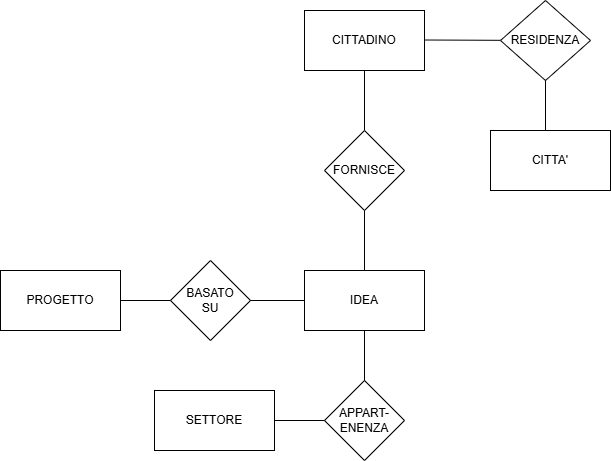
\includegraphics[width=0.8\textwidth]{images/SCHELETRO_CITTADINO.drawio.png}
    \caption{Schema scheletro per i cittadini}
    \label{fig:schema-sostenibilita}
\end{figure}

%--------------------------------ANALISI REQUISITI E SCHEMA SCHELETRO AZIENDA PRIVATA -----------------------------------------------

\newpage
\subsection{Analisi requisiti e schema scheletro per le Aziende Private}

\begin{longtable}{|p{3cm}|p{6.5cm}|p{2.5cm}|p{3cm}|}
\hline
\textbf{Termine} & \textbf{Descrizione} & \textbf{Sinonimi} & \textbf{Collegamenti} \\
\hline
\endfirsthead

\hline
\textbf{Termine} & \textbf{Descrizione} & \textbf{Sinonimi} & \textbf{Collegamenti} \\
\hline
\endhead

Azienda privata & Attore identificato da attributi come Partita IVA, ragione sociale e settore di attività. Ha il compito di produrre beni e servizi per la comunità. & Impresa, Organizzazione economica & Progetto, Città, Certificato \\
\hline

Progetto & Iniziativa che può essere avviata da un’azienda solo se in possesso della certificazione sostenibile. Mira alla creazione di un prodotto o servizio. & Iniziativa, Piano & Azienda \\
\hline

Certificazione sostenibile & Documento rilasciato dalla pubblica amministrazione che attesta la coerenza del progetto aziendale con i principi di innovazione e sostenibilità. & Certificato, Attestazione & Azienda \\
\hline

Città & Contesto urbano inteso sia come spazio fisico sia come organizzazione sociale, destinatario dei prodotti e servizi aziendali. & Sistema urbano, Comunità & Azienda \\
\hline

\caption{Glossario dei concetti relativi alle aziende nel sistema urbano sostenibile}
\label{tab:glossario-aziende}
\end{longtable}

\begin{figure}[H]
    \centering
    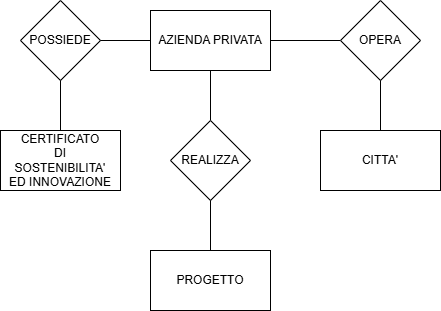
\includegraphics[width=10cm]{images/SCHEMA_SCHELETRO_AZIENDA.drawio.png}
    \caption{Schema scheletro per le aziende private}
    \label{fig:schema-sostenibilita}
\end{figure}

%--------------------------------ANALISI REQUISITI E SCHEMA SCHELETRO ENTE PUBBLICO -----------------------------------------------

\newpage
\subsection{Analisi requisiti e schema scheletro per gli Enti pubblici}

\begin{longtable}{|p{3cm}|p{6.5cm}|p{2.5cm}|p{3cm}|}
\hline
\textbf{Termine} & \textbf{Descrizione} & \textbf{Sinonimi} & \textbf{Collegamenti} \\
\hline
\endfirsthead

\hline
\textbf{Termine} & \textbf{Descrizione} & \textbf{Sinonimi} & \textbf{Collegamenti} \\
\hline
\endhead

Ente Regolatore & Attore identificato da codice univoco, settore di attività e residenza. Ha il compito di emettere certificati per i progetti. & Pubblica amministrazione & Città, Certificato \\
\hline

Certificato & Documento che rappresenta le competenze per produrre uno specifico progetto  & Attestato, documento & Ente Regolatore, Progetto \\
\hline

Ente Produttore & Attore identificato da codice univoco, settore di attività e residenza. Ha il compito di produrre i progetti per il miglioramento della propria città. & Impresa pubblica & Città, Progetto \\
\hline

Progetto & Iniziativa concreta derivata da un’idea selezionata, finalizzata alla realizzazione di un prodotto o servizio sostenibile. & Proposta, Iniziativa & Ente Produttore, Certificato \\
\hline

Città & Contesto urbano inteso sia come spazio fisico sia come organizzazione sociale, destinatario dei prodotti e servizi aziendali. & Sistema urbano, Comunità & Ente Regolamentatore, Ente Produttore \\
\hline

\caption{Glossario dei concetti relativi agli enti pubblici nel sistema urbano sostenibile}
\label{tab:glossario-enti}
\end{longtable}

\begin{figure}[H]
    \centering
    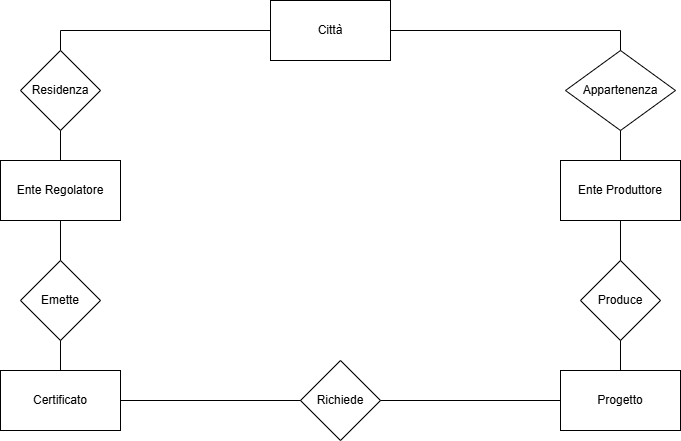
\includegraphics[width=15cm]{images/SchemaScheletroEnte.drawio}
    \caption{Schema scheletro per gli enti pubblici}
    \label{fig:schema-sostenibilita}
\end{figure}

\end{document}


%All other official TU Delft colours
\definecolor{donkerblauw}{RGB}{12, 35, 64}
\definecolor{turkoois}{RGB}{0, 184, 200}
\definecolor{blauw}{RGB}{0, 118, 194}
\definecolor{paars}{RGB}{111, 29, 119}
\definecolor{roze}{RGB}{239, 96, 163}
\definecolor{framboos}{RGB}{165, 0, 52}
\definecolor{rood}{RGB}{224, 60, 49}
\definecolor{oranje}{RGB}{237, 104, 66}
\definecolor{geel}{RGB}{255, 184, 28}
\definecolor{lichtgroen}{RGB}{108, 194, 74}
\definecolor{donkergroen}{RGB}{0, 155, 119}
%You can use these to change the hyperlink colour or the colour of the header or whatever. Glück Auf!